\documentclass[12pt,A4paper,oneside]{amsart}

%\usepackage{color,graphicx}
%\usepackage{mathrsfs,amsbsy}
\usepackage{bm}
\usepackage{booktabs}
\usepackage{ctex}
\usepackage{amssymb}
\usepackage{amsmath}
\usepackage{amsfonts}
\usepackage{array}
\usepackage{fancyhdr}
\usepackage{hhline}
\usepackage[unicode, bookmarksnumbered]{hyperref}	% 启动超链接和 PDF 文档信息所需
\usepackage{graphicx}
\usepackage{amsthm}
\usepackage{enumerate}
\usepackage{tikz}
\usetikzlibrary{shapes.geometric, arrows}
\usepackage[mathscr]{eucal}
\usepackage{mathrsfs}
\usepackage{verbatim}
\usepackage{wrapfig}
\usepackage{geometry} %调整页面的页边距
\usepackage{pifont}
\geometry{left=2.5cm,right=2.5cm,top=2cm,bottom=2cm}%具体的页边距设置
%\usepackage[notcite,notref]{showkeys}

% showkeys  make label explicit on the paper

%\makeatletter
%\@namedef{subjclassname@2010}{%
%  \textup{2010} Mathematics Subject Classification}
%\makeatother

\numberwithin{equation}{section}

\theoremstyle{plain}
\newtheorem{theorem}{Theorem}[section]
\newtheorem{lemma}[theorem]{Lemma}
\newtheorem{proposition}[theorem]{Proposition}
\newtheorem{corollary}[theorem]{Corollary}
\newtheorem{claim}[theorem]{Claim}
\newtheorem{defn}[theorem]{Definition}
\newtheorem{example}[theorem]{Example}

\theoremstyle{plain}
\newtheorem{exercise}{Exercise}[section]

\theoremstyle{plain}
\newtheorem{thmsub}{Theorem}[subsection]
\newtheorem{lemmasub}[thmsub]{Lemma}
\newtheorem{corollarysub}[thmsub]{Corollary}
\newtheorem{propositionsub}[thmsub]{Proposition}
\newtheorem{defnsub}[thmsub]{Definition}

\numberwithin{equation}{section}


\theoremstyle{remark}
\newtheorem{remark}[theorem]{Remark}
\newtheorem{remarks}{Remarks}
\newtheorem{ex}[theorem]{Exercise}
\newtheorem{question}[theorem]{Question}
\newtheorem{hint}[theorem]{Hint}

\newcommand*{\thick}[1]{\text{\boldmath$#1$}}
\newcommand*{\cir}[1]{\;$\ding{19#1}$\;}%临时使用
\newcommand*{\norm}[1]{\lVert#1\rVert}

%\renewcommand\thefootnote{\fnsymbol{footnote}}
%dont use number as footnote symbol, use this command to change

\DeclareMathOperator{\supp}{supp}
\DeclareMathOperator{\dist}{dist}
\DeclareMathOperator{\vol}{vol}
\DeclareMathOperator{\diag}{diag}
\DeclareMathOperator{\tr}{tr}


\begin{document}

\title[]{\LARGE 椭圆模函数理论笔记}


\author[]{\large 周潇翔}
\address{School of Mathematical Sciences\\
University of Science and Technology of China\\
Hefei, 230026\\ P.R. China\\}
\email{xx352229@mail.ustc.edu.cn}
\maketitle




\begin{abstract}
这篇文章是我看书\cite{klein1892vorlesungen}时的一些笔记整理,也借此机会欢迎大家一起来看这本书.其中Question是我所困惑的地方,感谢大家替我解答疑惑.
\end{abstract}




%%%%%%%%%%%%%%%%%%%%%%%%%%%%%%%%%%%%%%%%%%%%%%%%%%%%%%%%%%%%%%%%%%%%%%%%%%%%%%%%%%%%%%%%%%%%%
我们知道,对于紧黎曼面,亏格为0即为黎曼球,亏格为1时有三种称呼:亏格为1的紧黎曼面、复椭圆曲线、复环面.为了分类复环面,我们引入模空间$\mathcal{H}/SL(2,\mathbb{Z})$,考察这上面的模形式,可以发现所有模形式的空间就是$\mathbb{C}[E_2,E_3]$.由于模空间$\mathcal{H}/SL(2,\mathbb{Z})$在紧化后同构于黎曼球,我们称某一个特定的同构(亚纯函数)$j(z)$为模不变量,这个不变量唯一决定了复环面的结构.其详尽的解释参考\cite[第二,八章]{Li2019modularform}

我们的故事就从这里开始.在本书中,我们会重新从代数(不变量)的角度来考察$E_2,E_3,j$等看似分析的对象,从而对这些对象有更本质的认识.(为什么这些对象有那么多代数性质,因为其本身就是代数的)[1.1-1.13].

作为另一个重要目的,我们想要通过分式线性变换化简一元四次方程
$$f(x)=ax^4+4bx^3+6cx^2+4dx+e=0$$
为了使理论简单,我们将其齐次化,考虑二元齐四次型
$$f(z_1,z_2)=az_1^4+4bz_1^3z_2+6cz_1^2z_2^2+4dz_1z_3^3+ez^4$$
在线性变换
$$\begin{pmatrix}
z_1 \\ z_2
\end{pmatrix}=A\begin{pmatrix}
z'_1 \\ z'_2
\end{pmatrix}$$
下的标准型.
我们将导出三种标准型:
\begin{equation*}
\begin{aligned}
f&=z_1(z_2-z_1)(Az_1+Bz_2)z_2\\
f&=z_2(4z_1^3-g_2z_1z_2^2-g_3z_2^3)\\
f&=M(z_1^4+z_2^4)+6Nz_1^2z_2^2
\end{aligned}
\end{equation*}
并讨论与之有关的不变量:$$(A,B,C;\;A,B,\Gamma;\;G_2,G_3;\;g_2,g_3;\;\Delta;\;J;\;M,N,\mu_1,\mu_2;\;\mu)$$
\begin{ex}
	这些变量是如何定义的?它们之间有哪些关系?哪些是绝对不变量?哪些是有理不变量?
\end{ex}
\begin{question}
	在\cite[Part I,1.12]{klein1892vorlesungen}中,第一段最后的a new pair of points是什么?
	
	附:这一节的目的在于导出第三种标准型.文中使用几何方法.第一段如下:\\
	Yet a third canonical-form of $f$ will be discussed, which we introduce here by using some geometrical theorems, as well as properties of the four-group. We use the known theorem, that two points on a line uniquely determine another pair of points on the line, which have the property that they harmonically separate the given pair. But one can split the quadruple of points corresponding to $f\left(z_{1}, z_{2}\right)=0$ in three ways into two pairs of points, and to each of these splittings, we may associate a new pair of points with the line.
\end{question}
接下来[1.14-2.4],作者通过对不变量
$$\omega=\int \frac{dy}{\sqrt{4y^3-g_2y-g_3}}$$(这个不变量具有很强的几何意义,是椭圆函数的周期)
乘上系数$\sqrt{g_3/g_2}$后成为只依赖于$J$的绝对不变量$\Omega$.(这里在$y$平面固定了一条闭曲线$\gamma$.事实上,$\omega$也依赖于闭曲线$\gamma$所在的同伦类)
\begin{remark}
	关于开根号的歧义性,请详见书中解释,大致原因是我们不考虑不变量$\omega,\Omega$的正负号.
\end{remark}
我们通过对两类椭圆积分的求导得到关于$\Omega$的常微分方程
$$\frac{d^2\Omega}{dJ^2}+\frac{1}{J}\cdot\frac{d\Omega}{dJ}+\frac{31J-4}{144J^2(J-1)^2}\cdot \Omega=0$$
通过对该常微分方程的分析,我们得到:$\Omega$在$J=0,1,\infty$(这三个点为分歧点)以外的地方解空间都是二维的(并且"关于$J$光滑变化"),可以写为
$$\Omega=m_1\Omega_1+m_2\Omega_2$$
\begin{remark}
	这里的$\Omega_1,\Omega_2$是某对"primitive periods"经过改造得来的,并不是任意的选取."primitive periods"是格点作为$\mathbb{Z}$-模的基,而两个"primitive periods"之间只差一个变换$A \in SL(2,\mathbb{Z})$.可以说我们总是要找最为canonical的代表元,这样的做法是自然的.
	%(之后为叙述方便,我们也称$\Omega_1,\Omega_2$为"primitive periods")
\end{remark}
接下来[2.5-2.14],我们就希望调查$\Omega$在$J=0,1,\infty$附近的行为.在此之前,我们还没有真正确定$\Omega_1,\Omega_2$(我们希望选取的$\Omega_1,\Omega_2$"关于$J$光滑变化".另一方面,$\Omega_1,\Omega_2$取值虽然已经被"primitive"限制,但是并不是唯一的).

在这个问题下,文中具体给出了一个canonical的$\Omega_1,\Omega_2$(此时作为J的函数),并开始讨论$\Omega_1,\Omega_2$在$J-$平面上的解析延拓,这样给出一个黎曼面:它是$\mathbb{C}$(严格地说,是$\mathbb{C}P^1$)上的一个分歧覆盖,在$0,1,\infty$上分歧,分歧指数分别是$6,4,\infty$.而且,我们有群$SL(2,\mathbb{Z})$在纤维上的可迁作用,在非分歧点上稳定子群平凡.$\Omega_1,\Omega_2$可以看成是该黎曼面上的亚纯函数.

既然讨论黎曼面,自然要讨论其在分歧点上的性质(逆时针绕一圈有什么变化).经计算得到得到的新的周期$\Omega_1',\Omega_2'$均满足
\begin{equation*}
\begin{aligned}
\begin{pmatrix}
\Omega_1'\\\Omega_2'
\end{pmatrix}
\end{aligned}=A\begin{aligned}
\begin{pmatrix}
\Omega_1\\\Omega_2
\end{pmatrix}
\end{aligned}
\end{equation*}
其中$A$为$$U=\begin{pmatrix}
1 & 1\\
-1& 
\end{pmatrix}(\text{在$0$处})\qquad
T=\begin{pmatrix}
 & 1\\
-1& 
\end{pmatrix}(\text{在$1$处})\qquad
S=\begin{pmatrix}
1 & 1\\
 & 1
\end{pmatrix}(\text{在$\infty$处})$$
注意到$T,S$生成群$SL(2,\mathbb{Z})$,故我们研究的黎曼面是连通的.

在这个过程中,我们也顺便得到了$\Omega_1,\Omega_2$在分歧点附近的形式.
\begin{remark}
	这里取的黎曼面是书中黎曼面的某个连通分支.
\end{remark}
\begin{question}
	在\cite[Part I,2.14]{klein1892vorlesungen}中,为了验证我们的计算,书中希望在三个分歧点处各做一次变换,从$(\omega_1,\omega_2)$到$(\omega_1+\omega_2,-\omega_1),(\omega_1-\omega_2,\omega_2),(\omega_1,\omega_2)$,回到最初的解析分支.问题是,$(\omega_1+\omega_2,-\omega_1)$到$(\omega_1-\omega_2,\omega_2)$这一步是怎么做到的?(似乎不是乘矩阵$T$)
\end{question}
\section{使用共形映照研究绝对不变量$\lambda,\mu,\omega$,以及$s$-函数[2.15-3.21]}
我们先导出第三个绝对不变量
$$\omega=\frac{\Omega_1}{\Omega_2}$$
并推导出它满足的ODE:
$$[\omega]_{J}:=\frac{\omega'''}{\omega'}-\frac{3}{2}\left(\frac{\omega''}{\omega'}\right)^2=\frac{4}{9J^2}+\frac{3}{8(1-J)^2}+\frac{23}{72J(1-J)}$$
可以发现它是某个特殊的Schwartzian $s$-函数.事实上,$\lambda,\mu$也是某个特殊的Schwartzian $s$-函数.这暗示着我们所研究的对象和三角形镶嵌有关.
\begin{remark}
	符号$[z]_{J}$在模形式中的意义,就目前理解,可以从恒等式
	$$[z]_{J}=\left[\frac{az+b}{cz+d}\right]_{J}$$
	观之.之后我们会使用这个恒等式得到一个\textbf{单值}的函数.
\end{remark}
回顾这些不变量之间的关系:
$$\lambda=-\left(\frac{\mu^2-1}{2\mu}\right)^2 \qquad J=\frac{4}{27}\frac{(\lambda+\lambda^{-1}-1)^3}{\lambda+\lambda^{-1}-2}$$
$$J=\frac{(\mu^4+\mu^{-4}+14)^3}{108(\mu^4+\mu^{-4}-2)^2}$$
这些看似杂乱无章的函数背后,隐藏着众多的奥妙.

我们接下来,将会将有理函数理解成$\mathbb{C} \times \mathbb{C}$中的黎曼面,两个投影映射自然给出这个黎曼面的两种覆叠(一个是单页覆叠,另一个一般是分歧覆叠).作为分歧覆叠,我们用连续可微曲线在$\mathbb{C}P^1$中连接所有分歧点的像,将$\mathbb{C}P^1$分为两个单连通区域,这样其原像将黎曼面分成一片一片的,投影之后看就将$\mathbb{C}$分成一片一片的.这个比喻不是很妥当,最好拿书中的图片一起解释,也可以参考\cite[p99,FIG.3-11.]{ahlfors1979complex}

这里最漂亮的,是我们用(复)分析的方式来研究一个代数的函数,得到的是初等几何的图像(引入射影几何).这个图像具有丰富的对称性(引入群,这里的代数来自最开始对象的代数性,并且最开始的函数内蕴着这样的对称性),给出了一个$\mathbb{C}P^1$的全等三角形镶嵌(引入曲率与面积,欧拉示性数).更一般地,我们可以从某个给定内角的$\mathbb{C}P^1$中的三角形开始,不断地进行反射操作,从而得到$\mathbb{C}P^1$的全等三角形镶嵌,反过来寻找这个镶嵌所对应的代数函数!


\begin{ex}
我们以习题的方式做一些对过往知识的回顾:
\begin{enumerate}
	\item 这是为了算函数$\mu(J)$的分支点.当$J'(\mu_0)=0$ or $\infty$时,求所有$J(\mu_0)$可能的值.
	\item 设$\mu=x+iy$.说明$$Im (\mu^4+\mu^{-4}) =0 \Longleftrightarrow xy(x+y)(x-y)(x^2+y^2-1)=0$$
	\item 你还记得世界上一共有多少种正多面体吗?请用Euler示性数和曲率这两种方法证明.
	\item $\mathbb{C}$的全等三角形镶嵌一共有多少种?[3.19]$\mathcal{H}$呢?[3.20]
\end{enumerate}
\end{ex}
反过来寻找的这个镶嵌所对应的代数函数,其实就是$j$-函数的反函数.
我们定义$j(\alpha,\beta,\gamma;-)$函数为这样一个亚纯函数:它将上半平面映为三个角为$\alpha \pi,\beta \pi, \gamma\pi$的圆弧段三角形.

我们通过复分析的方法得到这个函数满足的微分方程:
$$[s]_J=\frac{1-\alpha^2}{2(J-1)^2}+\frac{1-\beta^2}{2J^2}+\frac{\alpha^2+\beta^2-\gamma^2-1}{2J(J-1)}$$
利用这个方程,我们猜出$\omega(\lambda)=s(0,0,0;\lambda)$.

最后,在去掉那些反函数非单值的情况后,我们利用$\alpha+\beta+\gamma-1$的符号的正负性将$s$-函数分为三类,这三类分别对应着我们熟悉的三个单连通黎曼面:$\mathbb{C}P^1,\mathbb{C},\mathcal{H}$.
\begin{figure}[th]
\begin{minipage}[t]{.49\textwidth}
	\centering
	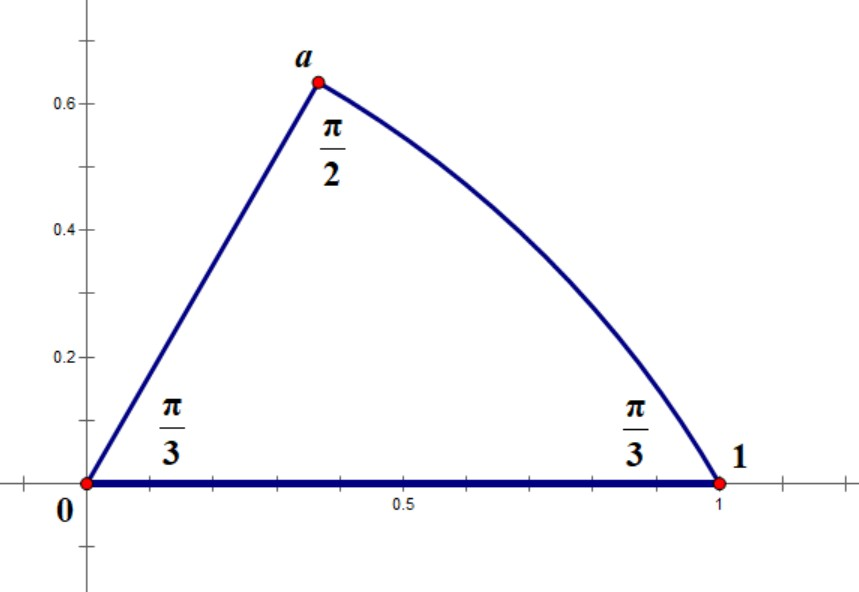
\includegraphics[width=.95\textwidth]{figures/triangle.jpg}\\
	\caption{}
	\label{fig1}
\end{minipage}
\end{figure}
\begin{ex}
	设$J(z)$是将图中三角形共形映至$-\mathcal{H}$,将$0,1,a$映至$0,\infty,1$的函数,求证:
	$$J(z)=\frac{z^3(z^3+8)^3}{64(z^3-1)^3}$$
\end{ex}
\begin{hint}
	考虑解析延拓,使用\cite{ahlfors1979complex}
\end{hint}
\begin{center}
	\begin{tabular*}{5cm}{c}
		\hline
	\end{tabular*}
\end{center}
鉴于我长时间没有更新,做个流程图来弥补一下,回顾下之前所了解到的内容.
\\


\tikzstyle{startstop} = [rectangle,rounded corners, minimum width=3cm,minimum height=1cm,text centered, draw=black,fill=red!30]
\tikzstyle{io} = [trapezium, trapezium left angle = 70,trapezium right angle=110,minimum width=3cm,minimum height=1cm,text centered,draw=black,fill=blue!30]
\tikzstyle{process} = [rectangle,minimum width=3cm,minimum height=0.5cm,text centered,text width =10cm,draw=black,fill=orange!30]

\tikzstyle{arrow} = [thick,->,>=stealth]
\tikzstyle{arrow2} = [thick,<->,>=stealth]
\begin{center}
\begin{tikzpicture}[node distance=1cm]
\node (start) [startstop,yshift=-0.6cm] {Start};
\node (input1) [process,below of=start,yshift=-0.6cm] {各类不变量};
\node (input2) [process,below of=input1,yshift=-0.6cm] {不变量直接的关系:特殊函数,三角镶嵌};
\node (input3) [process,below of=input2,yshift=-1cm] {特殊函数之间的比较:以模方程与正二十面体方程的类比为例};
\draw [arrow] (start) -- (input1);
\draw [arrow] (input1) -- (input2);
\draw [arrow] (input2) -- (input3);
\end{tikzpicture}
\end{center}
所以接下来的事情[4.1-4.13]就是:将模方程与正二十面体方程进行类比啦!

回顾模方程
$$J:J-1:1=g_2^3(\omega_1,\omega_2):27g_3^2(\omega_1,\omega_2):\Delta(\omega_1,\omega_2)$$
正二十面体方程
$$J:J-1:1=H^3(\zeta_1,\zeta_2):-T^2(\zeta_1,\zeta_2):1728f^5(\zeta_1,\zeta_2)$$
你可以自行比较方程的形式,还有它们对应的$s$-函数:
$$\omega(J)=s\left(\frac{1}{2},\frac{1}{3},\frac{1}{\infty};J\right)\qquad\zeta(J)=s\left(\frac{1}{2},\frac{1}{3},\frac{1}{5};J\right)$$
更为神奇的是,我们在较为复杂的计算后发现,在模方程中(在不计较常数的情况下),$g_2$是$\log \Delta$的Hessian矩阵的行列式,$g_3$是向量值函数$g_2,g_3$的Jacobi矩阵的行列式.这对正二十面体方程也是成立的:$H$是$f$的Hessian矩阵的行列式,$T$是向量值函数$f,H$的Jacobi矩阵的行列式.

另一方面,当我们引入新的函数$X=g_2/g_3$时,$g_2,g_3,\Delta$就有只依赖于$X,J$(不依赖$\omega_1,\omega_2$)的表达:
$$g_2=\frac{3^3J}{X^2(J-1)}\qquad g_3=\frac{3^3J}{X^3(J-1)}\qquad \Delta=\frac{3^9J^2}{X^6(J-1)^3}$$
我们使用Taylor展开来算函数$g_2,g_3,\Delta$的零点位置.这之后,我们想要进行更为深入的比较.
\pagebreak
\begin{question}
	下面这个似乎是一道GRE阅读题..当然,你可以参考\cite[I.Chapter 4]{klein2003lectures}.
	
	阅读下面两段摘自\cite[I,4.10]{klein1892vorlesungen}的段落,回答以下问题:
	\begin{enumerate}
		\item 第一段的"domain of rationality"是什么意思?
		\item 翻译倒数第二句话.
	\end{enumerate}
	It will be extremely rich in consequences, if we now carry through the comparison of
	the two oft-mentioned equations also for the domain of the Galois theory. It nevertheless requires a preliminary investigation, to see in what sense the definitions of the
	above mentioned theory of algebraic equations, to which they primarily refer, can be carried over to the transcendental modular equation. First and foremost, we are concerned in this regard with the concept of the \underline{\textit{domain of rationality}} and the \textit{group of the equation}, whereby we must especially make ourselves aware of their double meaning
	for such equations, which, besides constant coefficients, even contain variable parameters. We may restrict ourselves to the case, that only one such parameter exists. In fact,
	our two equations contain only one variable parameter, the quantity $J$.
	
	The domain of rationality of an "algebraic" equation of this kind will, aside from
	possible numerical quantities, in any case, still contain the parameter. Accordingly, a rationally-known quantity, insofar as it is not constant, must contain the variable
	parameter in rational fashion. And now it is here, where the special position of the parameter vis-a-vis constant quantities, grounded in its free variability, has, as consequence, a different kind of definition of the words domain of rationality. \textbf{Either one makes the requirement, to contain the parameter rationally, lets it go at that,
		and explains by \textit{rationally-known each rational function of the parameter in the sense of the theory of functions, irrespective of whether numerical irrationalities are contained in the expression of this function or not}; or else one calls rationally known a rational function of the parameter only if its coefficients are, \textit{in the arithmetical sense, rationally combined from a well-determined circle of numerically given numbers.}} We call the first standpoint, according to its nature, \textit{the function-theoretic}, and the latter, which is the more encompassing, \textit{the arithmetic}.

\end{question}

由于我对这两段内容的无知,我们暂且先跳过第4节.(后面部分看标题似乎是提出了群论方向的基本问题与函数论方向的基本问题)第五节的前半部分[5.1-5.6???]是我们早已熟悉的内容:不变量的解析表达.所以这里的重点是看它怎么与之前的不变量定义等价的.

而后半部分则引入了两类函数:$\sigma$-函数与$\vartheta$-函数.

$\sigma$-函数的构造很有意思:我们考虑$\wp$函数的原函数
$$Z(u):=\int \wp(u)du=-\frac{1}{u}+\frac{g_2}{2^2 \cdot 3 \cdot 5}u^3+\cdots$$
为方便起见取常数为0.注意这里的原函数是全局范围良定的亚纯函数,但不再是双周期函数.再考虑该函数的"原函数"
$$\int Z(u)du=- \log u+\frac{g_2}{2^4 \cdot 3 \cdot 5}u^4+\cdots$$
(为方便起见取常数为0)注意由于$Z$函数中$\frac{1}{u}$的存在,这里的函数不再是单值函数:每绕某个格点逆时针绕一圈,函数值减少$2\pi i$.为了得到单值函数,我们再取指数处理:
$$\sigma(u):=\exp\left(-\int Z(u)du\right)=u-\frac{g_2}{2^4 \cdot 3 \cdot 5}u^5-\cdots$$
这样我们终于得到一个全局良定的全纯函数$\sigma(u)$,零点值恰好为所有格点,并且满足一定的恒等式,比较特殊的如:
$$\sigma (u+\omega_1)=-e^{\eta_1(u+\omega_1/2)}\sigma(u) \qquad \sigma (u+\omega_2)=-e^{\eta_2(u+\omega_2/2)}\sigma(u)$$

$\vartheta$-函数???我还没看.

在这个过程中我们重新认识了椭圆积分.其中第一类椭圆积分是$\wp$的反函数,某种意义上就是从复椭圆曲线到复环面的具体构造.另外,复椭圆曲线上的亚纯函数域即为$\mathbb{C}(\wp(y),\wp'(y))$,这可以从以下公式中看出:
$$\wp(y)=u \qquad \wp'(y)=\sqrt{4u^3-g_2y-g_3}$$
而第二类椭圆函数则在$\sigma$-函数的构造中大显身手.注意到
$$Z(u)=\int \wp(u)du=\int \frac{udu}{\sqrt{4u^3-g_2u-g_3}}$$
就是第二类椭圆函数.

那接下来的内容就得等我拿到这两本书的邮寄了.???是之后会补的部分,哈哈.(然而已经两年没有更新了,而且预计在可见的将来也不会更新2333,书\cite{klein2003lectures}的内容已经写成本科毕业论文--读书笔记了.)
\begin{equation*}
\begin{aligned}
内容...
\end{aligned}
\end{equation*}
%%%%%%%%%%%%%%%%%%%%%%%%%%%%%%%%%%%%%%%%%%%%%%%%%%%%%%%%%%%%%%%%%%%%%%%%%%%%%%%%%%%%%%%%%%%%%





%%%%%%%%%%%%%%%%%%%%%%%%%%%%%%%%%%%%%%%%%%%%%%%%%%%%%%%%%%%%%%%%%%%%%%%%%%

\bibliography{reference}	
\bibliographystyle{plain}




%%%%%%%%%%%%%%%%%%%%%%%%%%%%%%%%%%%%%%%%%%%%%%%%%%%%%%%%%%%%%%%%%%%%%%%%%%%%%%%%%%%%%%%%%%%%%%%







\end{document}




